\section{Appendices}
%\appendix
\begin{appendices}
\section{Audio pre-processing code}


The following code records, processes and then plays the double integrated and square-rooted output. Additional code sources are available on the github repository for this project at \url{https://github.com/SnoWHandS/Directional_Audio_System}.

\begin{lstlisting}[caption={Record, process and play julia code}\label{lst:juliarecProPly},language=julia, style=jlcodestyle]

#Developed by Dillon Heald for use with a directional ultrasonic speaker array
#Date: April 2020



using PortAudio, Statistics, PyPlot, FFTW

stream = PortAudioStream(1, 1, blocksize=1024)

offset = 20

A = 1750                       #Amplitude multiple for final output signal
sample_rate = 44100
Nseconds = 10
N = Nseconds * sample_rate
Δt=1/sample_rate                 #seconds: inverse of sample rate
t=(0:N-1)*Δt                    #time axis def
#Define f_axis
Δf=1/(N*Δt)
f=0:(N-1)*Δf
#create array of freq values stored in f_axis. First element maps to 0Hz
if mod(N,2)==0    # case N even
    f_axis = (-N/2:N/2-1)*Δf;    
else   # case N odd
    f_axis = (-(N-1)/2 : (N-1)/2)*Δf; 
end

#Function for integrating a signal via Riemann sums
function integrate(x, Δt)
    N=length(x)
    y=zeros(N);
    for n=2:N
        y[n]=x[n-1]*Δt + y[n-1]
    end
    return y
end

#Function for high pass filtering a time domain
function hpf(in_signal, time_step, cutoff_freq)
    out_signal = Array{Float64}(undef, length(in_signal));
    RC = 1/(2*pi*cutoff_freq);
    a = RC/(RC + time_step);
    out_signal[1] = in_signal[1]
    for i = 2:length(in_signal)
        out_signal[i] = a*(out_signal[i-1] + in_signal[i] - in_signal[i-1]);
    end;
    return out_signal;
end;

println("Recording $(Nseconds) seconds of sampled audio")

buf_read = read(stream,N)
buf = buf_read

println("Processing $(Nseconds) seconds of sampled audio")

#Shift function to above 0 for preprocessing
buf = buf_read

#integrate once with function centered at 0
y1 = integrate(buf, Δt)
Y1 = fft(y1)
y1_filt = hpf(y1,Δt,80)
Y1_filt = fft(y1_filt)
#integrate twice
y2 = integrate(y1_filt, Δt)
Y2 = fft(y2)
y2 = hpf(y2,Δt,160)
y2_filt = hpf(y2,Δt,160)
Y2_filt = fft(y2_filt)

#Shift function to above 0 for preprocessing
buf = y2_filt.-minimum(y2_filt)

#Perform a square root of the samples
buf = sqrt.(buf)

close("all")
figure(2)
nStart=Int(round(Δt/Δt))
nEnd=Int(round(N*Δt/Δt))
subplot(3,1,1)
plot(t[nStart:nEnd],y1_filt[nStart:nEnd])
xlabel("y1 output")
subplot(3,1,2)
plot(f_axis,abs.(fftshift(Y1)))
xlabel("FFT of Y1")
subplot(3,1,3)
plot(f_axis,abs.(fftshift(Y1_filt)))
xlabel("FFT of Y1 filtered")

figure(3)
nStart=Int(round(Δt/Δt))
nEnd=Int(round(N*Δt/Δt))
subplot(3,1,1)
plot(t[nStart:nEnd],y2_filt[nStart:nEnd])
xlabel("y2 output")
subplot(3,1,2)
plot(f_axis,abs.(fftshift(Y2)))
xlabel("FFT of Y2")
subplot(3,1,3)
plot(f_axis,abs.(fftshift(Y2_filt)))
xlabel("FFT of Y2 filtered")

#filter away DC
buf = hpf(buf,Δt,75)

#shift center back to 0 and amplify to be audible
buf = A*buf

BUF = fft(buf)
BUF_READ = fft(buf_read)

figure(1)
nStart=Int(round(0.0025/Δt))        #Artifact with samples before 0.0025s = 2.5ms
nEnd=Int(round(N*Δt/Δt))
subplot(4,1,1)
plot(t[nStart:nEnd],buf[nStart:nEnd])
xlabel("envelope output")
subplot(4,1,2)
plot(t[nStart:nEnd],buf_read[nStart:nEnd])
xlabel("original output")
subplot(4,1,3)
plot(f_axis,abs.(fftshift(BUF_READ)))
xlabel("FFT of original")
subplot(4,1,4)
plot(f_axis,abs.(fftshift(BUF)))
xlabel("FFT of output")


println("Playing $(Nseconds) seconds of sampled audio")

write(stream, buf)
close(stream)

\end{lstlisting}

\section{Project management \& planning}
The following project planning was performed following initial proposal of the project. By mid March, the Covid-19 pandemic struck South Africa and resulted in national lock down. This altered the scope of the project and shifted timelines, thus the date information is not accurate; however, the work flows remained the same albeit shifted and reduced in scope to account for the disruption.
\subsection{Work breakdown structure}
\begin{figure}[ht]
    \centering
    \includegraphics[width=\textwidth]{Figures/Work_Breakdown_Structure_1000dpi.png}
    \caption{Work breakdown structure for the the directional audio system}
    \label{fig:wbs}
\end{figure}
\newpage
\subsection{Gantt chart}
\begin{figure}[ht]
    \centering
    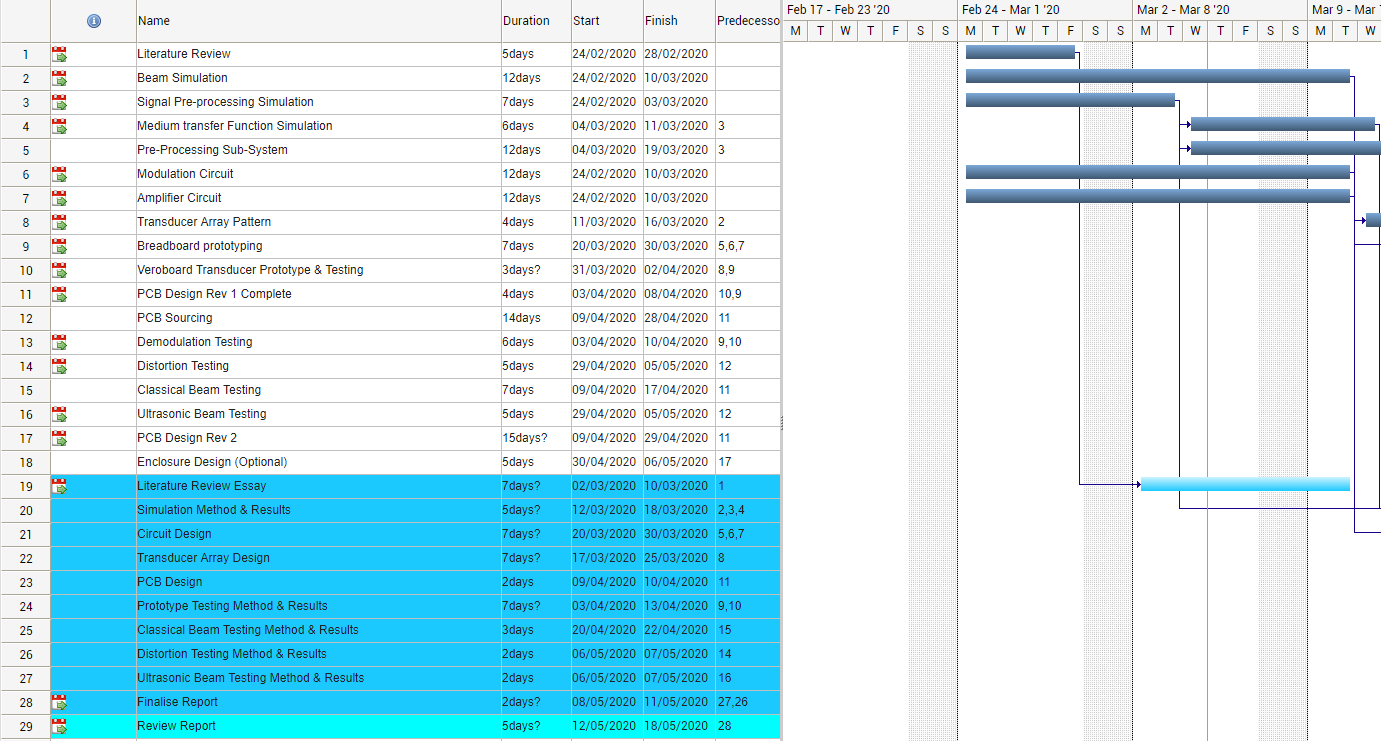
\includegraphics[width=\textwidth]{Figures/Gantt1.PNG}
    \caption{Gantt chart part 1}
    \label{fig:gantt1}
\end{figure}
\begin{figure}[ht]
    \centering
    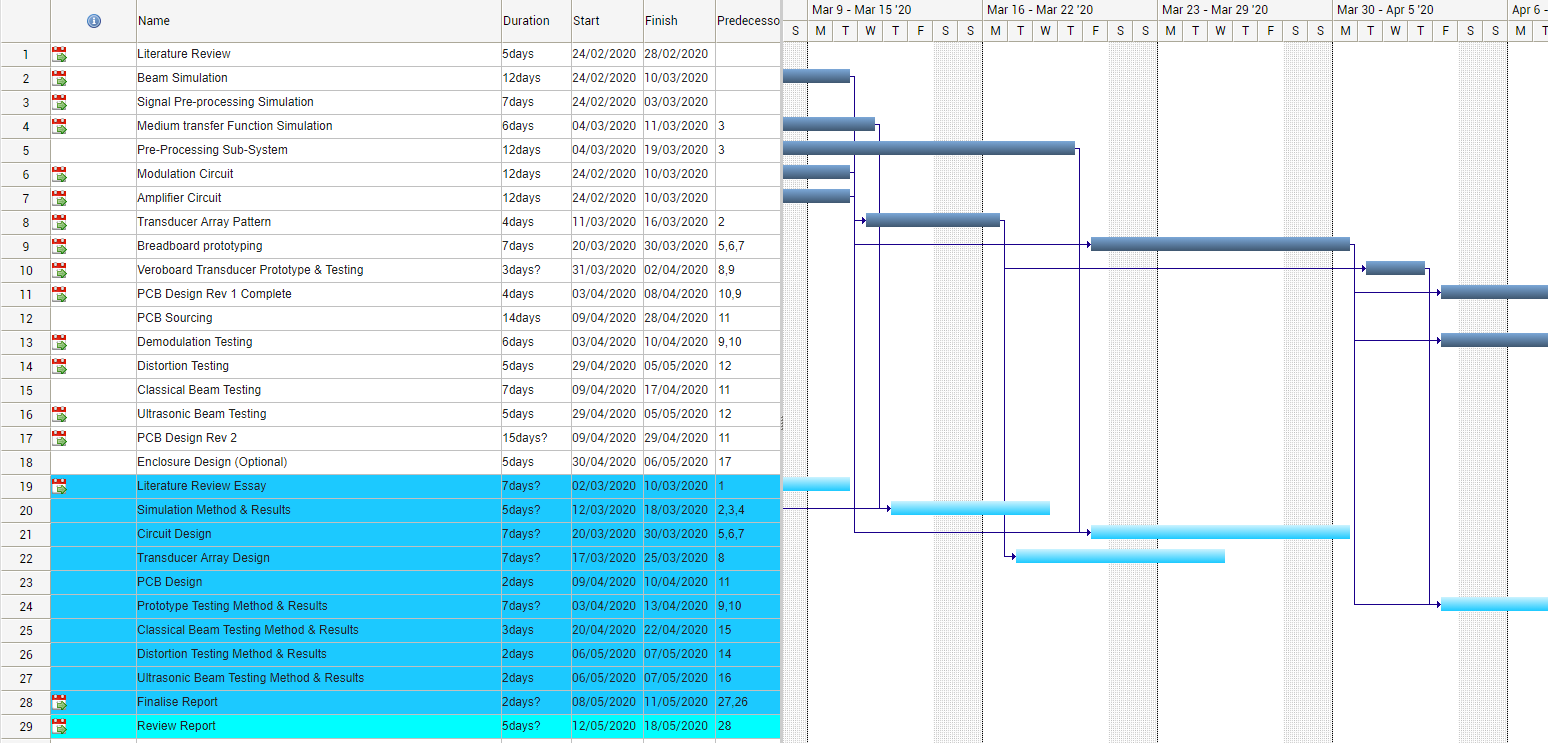
\includegraphics[width=\textwidth]{Figures/Gantt2.PNG}
    \caption{Gantt chart part 2}
    \label{fig:gantt2}
\end{figure}
\begin{figure}[ht]
    \centering
    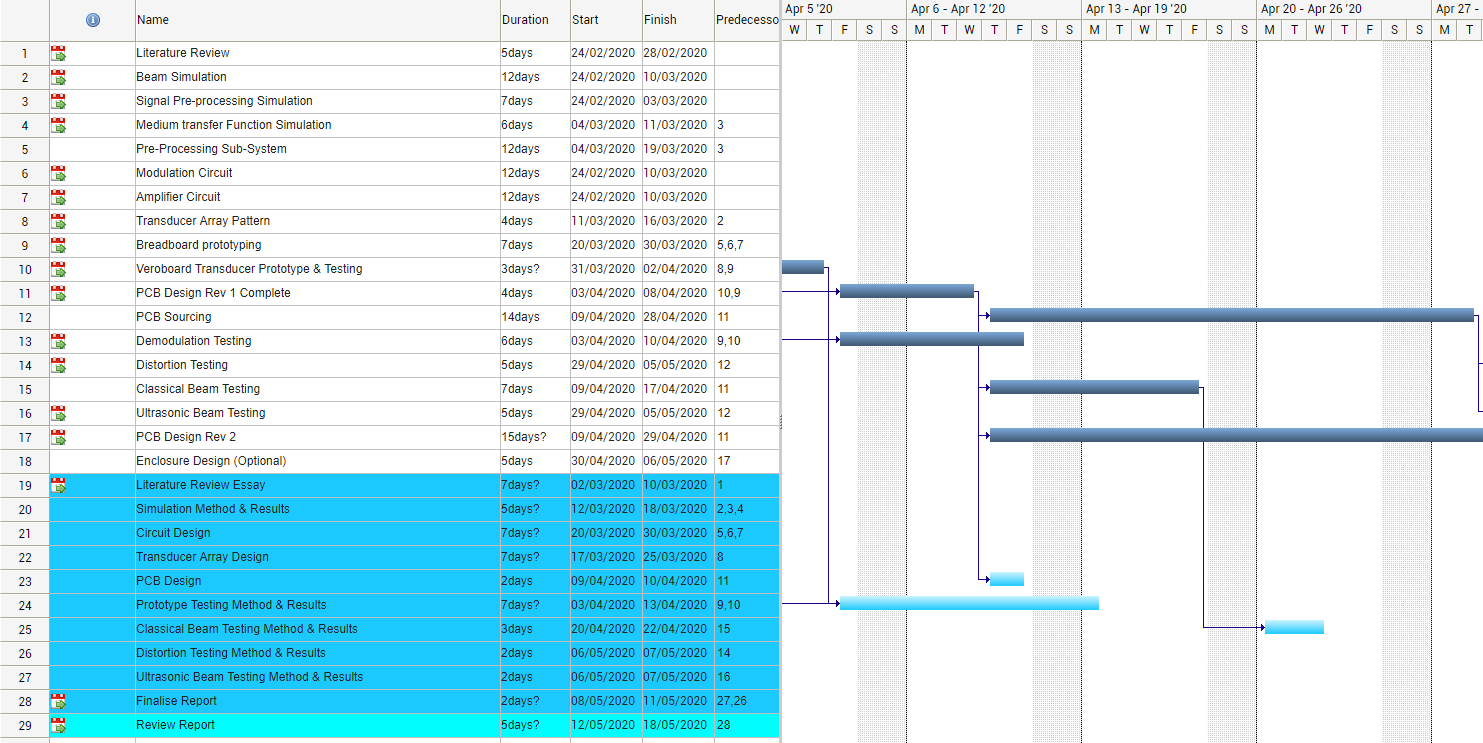
\includegraphics[width=\textwidth]{Figures/Gantt3.PNG}
    \caption{Gantt chart part 3}
    \label{fig:gantt3}
\end{figure}
\begin{figure}[ht]
    \centering
    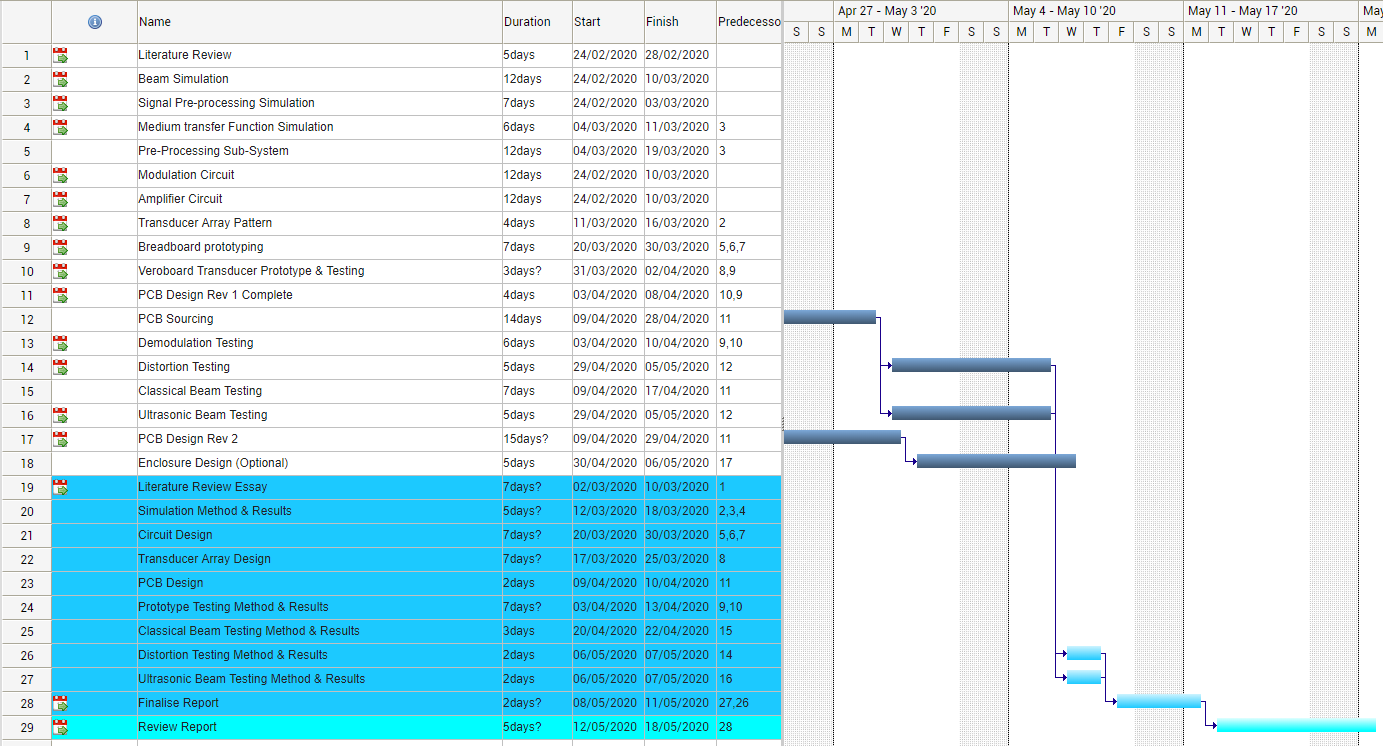
\includegraphics[width=\textwidth]{Figures/Gantt4.PNG}
    \caption{Gantt chart part 4}
    \label{fig:gantt4}
\end{figure}

\end{appendices}
